\begin{figure}[t]
\centering
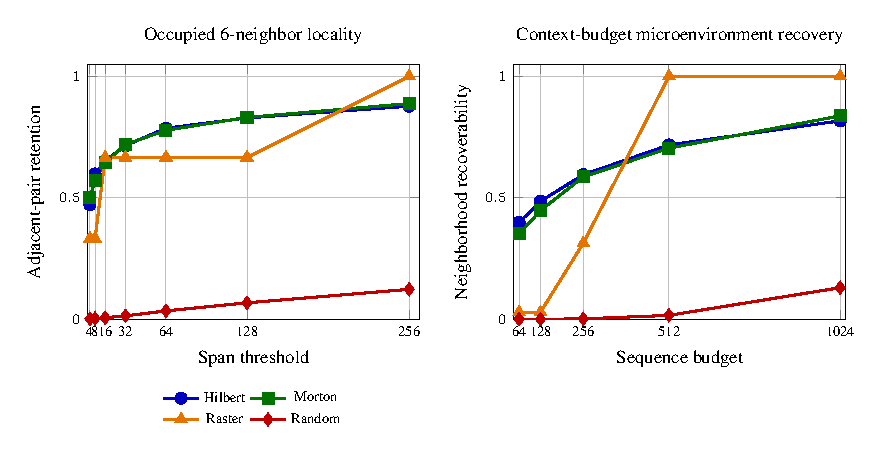
\includegraphics[width=0.98\linewidth]{../figure_assets/probe_curves/probe_curves.pdf}
\caption{Computed probe curves. Left: retention of occupied 6-neighbor pairs as the allowable serialized span increases. Right: recovery of mixed-channel local environments as the available sequence budget increases. Hilbert and Morton behave smoothly under tight budgets, raster shows a plane-boundary cliff, and random order destroys locality.}
\label{fig:probe-curves}
\end{figure}
